% Imporditud: tools/import_eksperimendid.py
% Allikas: Eesti füüsikaolümpiaadi eksperimendi ülesannete
%   kogu (Rael Kalda, 2023), ülesanne Ü121, lahendus L121.
\setAuthor{Hans Daniel Kaimre}
\setRound{lõppvoor}
\setYear{2020}
\setNumber{P E2}
\setDifficulty{3}
\setTopic{elektriahelad}
\setVahendid{must kast, millest väljub kolm juhet, ühendusjuhtmed, multimeeter. Takistite väärtused on sellised, et võib eeldada, et multimeeter töötab ideaalse amper- ning voltmeetrina}
\setPunktid{12}
\setAllikas{Eksperimendi kogu Ü121, lahendus lk 96}
\setLahendusseis{toores}

\prob{Must kast}
Teha kindlaks mustas kastis (skeem joonisel) olevate komponentide väärtused
(patarei pinge $U$, takistused $R_1$, $R_2$, $R_3$). Multimeetrit saab
ühendada punktides R (roosa), S (sinine) ja P (pruun). Patarei sisetakistusega
mitte arvestada.

\begin{center}
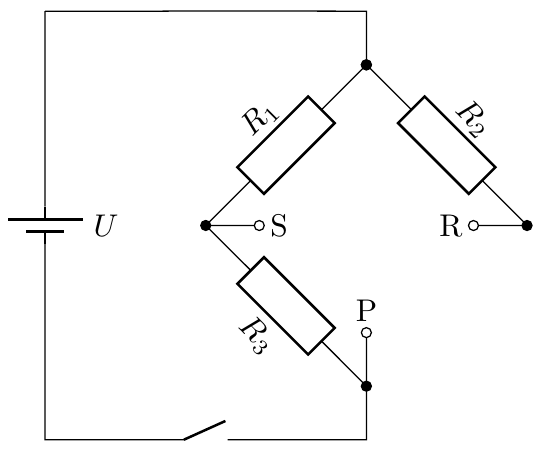
\includegraphics[width=0.40\linewidth]{2020-v3g-pe2-yl.png}
\end{center}

\textbf{NB!} Kui mõõtmisi parasjagu ei teostata, tuleks seade hoida
\textit{OFF}-asendis, et vältida patarei tarbetut tühjenemist.

\hint

\solu
Paneme esmalt tähele, et kuna voltmeetrit võib käsitleda ideaalsena, siis ühendades multimeetri voltmeetrina klemmide R ja P vahele, on pingelang takistil $R_2$ marginaalne. Järelikult URP = U . Ühendades multimeetri ampermeetrina punktide S ja P vahele, läbib vool ainult takistit $R_1$, seega Ohmi seadusest

$R_1$ = U = URP . ISP ISP

Kui multimeeter ühendada ampermeetrina klemmide P ja R vahele, on pinge $R_2$ klemmidel võrdne pingega patarei klemmmidel ning

$R_2$ = URP . IRP

Siit edasi on kaks erinevat lahenduse võimalust: multimeetri oommeetri funktsiooni kasutades (a) ning seda funktsiooni kasutamata (b). a) Ühendades lüliti lahti (asendisse OFF), saame mõõta multimeetri oommeetri funktsiooniga otse takistusi. Niimoodi saamegi, et:

RSP = $R_3$

b) Selleks, et leida $R_3$ takisti väärtus ainult volt- ning ampermeetrit kasutades, pa-

neme tähele et kui takistit $R_2$ vool ei läbi, peab voolutugevus takistites $R_1$ ja $R_3$

olema võrdne, seega

USR = USP $\Rightarrow$ $R_3$ = USP $R_1$ $R_1$ $R_3$ USR

Lahendusi on muidugi veel, kuna saame teha 7 üksteisest sõltumatut (2 pinget, 2

takistust ning 3 voolutugevust) erinevat mõõtmist ning tundmatuid on 4, kuid ülal-

toodud variandid on žürii arvates lihtsaimad. Erinevad võimalikud mõõtmistule-

mused on järgmised: URP = 3,25 V, USR = 2,05 V, USP = 1,204 V, ISP = 6,37 mA,

ISR = 4,77 mA, IRP = 13,5 mA, RSP = 300 $\Omega$, RSR = 750 $\Omega$, RRP = 1050 $\Omega$. Nen-

dest tulemustest saame:

U = URP = 3,25 V

$R_1$ = URP = 3,25 V = 510 $\Omega$ ISP 6,37 mA

$R_2$ = URP = 3,25 V = 240 $\Omega$ IRP 13,5 mA

$R_3$ = RSP = 300 $\Omega$
\probend
